\chapter{复微积分}
\begin{introduction}
    \item 复变函数
    \item 解析函数
    \item 多值函数
    \item 复变函数的积分
\end{introduction}
\section{复变函数}
    \subsection{复变函数的定义}
        与实数集上的实变函数相对应,复变函数就是由复数集到复数集的映射.\par
        \begin{definition}[复变函数]\label{def:complex_function}
            对于映射$f: \mathbbm{C} \to \mathbbm{C}$,写作$f(z)=w$,称为复变函数.
        \end{definition}

        复变函数是平面到平面的映射,它将复平面$z$上的点逐一映射到复平面$w$上.
        对于任意复数$z \in \mathbbm{C}$,我们可以将其写作如下形式$z = x + iy,(x,y \in \mathbb{R})$,
        于是我们也可以将复变函数$f(z) = w$写作两个实变函数的形式:
        \begin{align}
            f(z) = u(x,y) + iv(x,y)
        \end{align}

        其中,$u(x,y)$和$v(x,y)$分别是$f(z)$的实部和虚部,点$(u, v)$为复平面$w$上的点.

    \subsection{复变函数的极限}
        \begin{definition}[复变函数的极限]\label{def:limits_of_complex_function}
            极限$lim_{z \to a}f(z) = w_0$表示对于任意实数$\epsilon > 0$,都存在一个实数$\delta > 0$,
            使得当$|z - a| < \delta$时,都有$|f(z) - w_0| < \epsilon$.
        \end{definition}

        \begin{definition}[复变函数的连续性]\label{def:continuity_of_complex_function}
                    同理,在$z = a$处如果有$lim_{z \to a}f(z) = f(a)$,则称$f$在$z = a$处连续.
                \end{definition}


\section{解析函数}

    \subsection{复变函数的微分}
        判断一个复变函数是否可微,我们有Cauchy-Riemann条件:
        \begin{theorem}[Cauchy-Riemann条件]\label{the:Cauchy-Riemann_condition}
            对于复变函数$f(z) = u(x,y) + iv(x,y)$,如果对于点$z_0$,有
            \begin{align}
                \frac{\partial u}{\partial x} = \frac{\partial v}{\partial y} \quad and \quad \frac{\partial u}{\partial y} = -\frac{\partial v}{\partial x}
            \end{align}
            $f$在$z = z_0$处才能可微.
        \end{theorem}

        注意$Cauchy-Riemann$条件仅是$f$可微的必要不充分条件,这里给出判断$f$可微的充要条件:
        \begin{theorem}\label{the:differentiability_of_complex_function}
            复变函数$f(z) = u(x, y) + iv(x, y)$在区域$G$上可微的充要条件为,$C-R$条件成立:
            \begin{align*}
                \frac{\partial u}{\partial x} = \frac{\partial v}{\partial y} \quad and \quad \frac{\partial u}{\partial y} = -\frac{\partial v}{\partial x}
            \end{align*}
            且在区域$G$上,$u$和$v$的一阶导存在且连续.
        \end{theorem}

        \begin{lemma}
            \label{lem:complex_function_differentiable_with_respect_to_z}
            当$f$可微时,$f$与$z^*$无关,即$\dfrac{df}{dz^*} = 0$.
        \end{lemma}
        \begin{proof}
            当$f$可微时,我们有$C-R$条件成立,于是有:
            \allowdisplaybreaks
            \begin{align*}
                \frac{df}{dz^*} &= \frac{\partial v}{\partial (-y)} - i \frac{\partial u}{\partial (-y)}\\
                &= -\frac{\partial v}{\partial y} + i \frac{\partial u}{\partial y}\\
                &= -\frac{\partial u}{\partial x} - i \frac{\partial v}{\partial x}\\
                &= \frac{\partial u}{\partial x} + i \frac{\partial v}{\partial x}
            \end{align*}
            于是我们得到:
            \begin{align*}
                \frac{\partial u}{\partial x} = \frac{\partial v}{\partial x} = \frac{\partial u}{\partial y} = \frac{\partial v}{\partial y} = 0
            \end{align*}
            即$\dfrac{f}{z^*} = 0$
        \end{proof}
        由引理\ref{lem:complex_function_differentiable_with_respect_to_z},我们可以给出另外一种判断$f$是否可微的方法:
        \begin{example}
            判断函数$f(z) = x^2 +2iy^2$的可微性
        \end{example}
        \begin{solution}
            我们有:
            \begin{align*}
                x = \frac{1}{2}(z + z^*), \quad y = \frac{1}{2i}(z - z^*)
            \end{align*}
            将$f(z)$使用$z$和$z^*$重写,
            \begin{align*}
                f(z) &= [\frac{1}{2}(z + z^*)]^2 + 2i[\frac{1}{2i}(z - z^*)]^2\\
                &= \frac{1}{4}(1 - 2i)(z^2 + z^{*2}) + \frac{1}{2}(1 + 2i)zz^*
            \end{align*}
            可以看到$f$与$z^*$有关,因此$f$不可微.
        \end{solution}

    \subsection{解析函数的定义}
        \begin{definition}[解析函数]\label{def:analytic_function}
            如果复变函数$f$在某一点$z_0$及其某一领域$U_0$上可微,则称$f$在$z_0$处解析.相应的,
            若$f$在某一区域$G \subset \mathbbm{C}$上均可微,则称$f$在$G$上解析.$f$解析的点称为正则点.
        \end{definition}
        \begin{definition}[奇点]\label{def:singular_point}
            若$f$在某一点$z_0$处不解析,但在$z_0$任一领域上均解析,则称$z_0$为$f$的奇点.
        \end{definition}
        \begin{theorem}[Laplace 方程]\label{the:Laplace_equation}
            若$f$在某一区域$G$上解析,则$f$在$G$上满足拉普拉斯方程:
            \begin{align*}
                \frac{\partial^2 u}{\partial x^2} + \frac{\partial^2 u}{\partial y^2} = 0. \quad \frac{\partial^2 v}{\partial x^2} + \frac{\partial^2 v}{\partial y^2} = 0
            \end{align*}
            由$C-R$条件易得.
        \end{theorem}

    \subsection{初等单值解析函数}
        \allowdisplaybreaks
        \begin{enumerate}
            \item 幂函数$z^n$\\
                当$n = 0,1,2,\dots$时,$z^n$在$\mathbbm{C}$上解析;且当$n = 1,2,\dots$时,$z^n$在$z = \infty$不解析.\\
                当$n = -1,-2,\dots$时,$z^n$在$z = 0$不解析,在包括$\infty$点在内的$\mathbb{C}$上除$0$外均解析.
            \item 多项式函数$P_n(z) = a_nz^n + a_{n-1}z^{n-1} + \dots + a_1z + a_0$
            \item 有理函数$R(z) = \dfrac{P_n(z)}{Q_m(z)}, \quad Q_m \neq 0$
            \item 指数函数$e^z$\\
                复指数函数具有周期性,这是实指数函数所不具有的,其周期为$2 \pi i$\\
                $e^z$在$\mathbb{C}$上解析,且在$z = \infty$不解析,证明如下:
                \begin{proof}
                    当$z$沿正实轴趋于无穷时,有$x \to \infty, \quad y = 0$,则$\lim_{z \to \infty}e^z = \lim_{x \to +\infty}e^x \to +\infty$;\\
                    而当$z$沿负实轴趋于无穷时,有$x \to -\infty, \quad y = 0$,则$\lim_{z \to -\infty}e^z = \lim_{x \to -\infty}e^x \to 0$;\\
                    可得$e^z$在$z = \infty$处不解析.
                \end{proof}
            \item 三角函数$\sin{z}, \cos{z}, \dots$\\
                复三角函数一般使用复指数函数来定义:
                \begin{align*}
                    \sin{z} &= \frac{e^{iz} - e^{-iz}}{2i}, \quad \cos{z} = \frac{e^{iz} + e^{-iz}}{2}
                \end{align*}
                在$z = \infty$处不解析.
            \item 双曲函数$\sinh{z}, \cosh{z}, \dots$\\
                复双曲函数同样由复指数函数定义.
                \begin{align*}
                    & \sinh{z} = \frac{e^z - e^{-z}}{2},& &\cosh{z} = \frac{e^z + e^{-z}}{2}, & \tanh{z} = \frac{\sinh{z}}{\cosh{z}}&\\
                    & \coth{z} = \frac{\cosh{z}}{\sinh{z}},& &\textnormal{sech}\,z = \frac{1}{\cosh{z}}, & \textnormal{csch}\,z = \frac{1}{\sinh{z}}&
                \end{align*}
                并且易知复双曲函数和复三角函数可以互相转化.
                \begin{align*}
                    \sinh{z} = -i\sin{iz}, \quad \cosh{z} = \cos{iz}, \quad \tanh{z} = -i\tan{iz}
                \end{align*}
        \end{enumerate}


\section{多值函数}

    \subsection{多值函数的定义}
        \allowdisplaybreaks
        \begin{definition}[多值函数]\label{def:multi_value_function}
            复数的幅角多值性导致某些函数将$z$平面上的点映射到$w$平面时,一个点会有多个点与之对应,我们就将这样的函数称为多值函数.
        \end{definition}

        事实上多值函数并不是函数,因为函数要求一一映射.我们主要研究的多值函数就是$f(z) = \sqrt{z - z_0}$和$f(z) = \ln{z}$,
        他们俩的多值性由下式给出:
        \begin{align}
            \label{eq:multi_value_function}
            &\sqrt{z - z_0} = \sqrt{|z - z_0|e^{i(\theta + 2n\pi)}} = \sqrt{|z - z_0|}e^{i\frac{\theta}{2}}e^{in\pi} = \pm \sqrt{|z - z_0|}e^{i\frac{\theta}{2}}\\
            &\ln{z} = \ln{|z|} + i(\theta + 2n\pi)
        \end{align}

        \begin{definition}[分支点(枝点)]\label{def:branch_point}
            如果多值函数的自变量$z$绕点$z_0$外任意闭合曲线$C$一圈后,多值函数的宗量(即$f(z) = \sqrt{z - z_0}$中的$z - z_0$)
            相位改变了$2\pi$,则称点$z_0$为多值函数的分支点.
        \end{definition}

        当我们做各种各样的计算时,肯定不希望出现多值的现象,从分支点的特性出发,你或许也能感觉到,只要避免自变量绕着分支点
        一直转圈圈,我们就能避免多值的出现.因此,我们可以通过限制自变量的取值范围来避免多值的出现,这就是多值函数的分支的概念.

    \subsection{黎曼面}
        \begin{figure}[htbp]
            \centering
            \begin{minipage}[t]{0.48\textwidth}
                \centering
                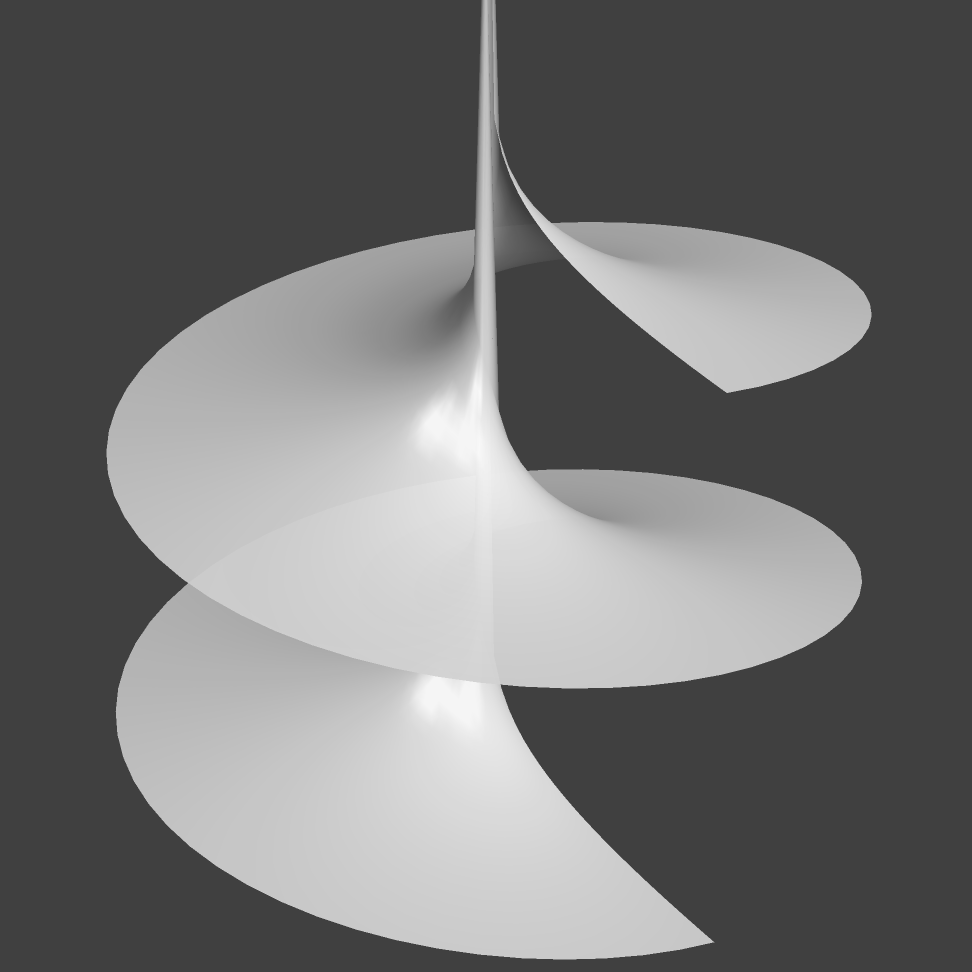
\includegraphics[width=0.9\textwidth]{RiemannSurface.png}
                \caption{$f(z) = \sqrt{z - z_0}$的黎曼面}
                \label{fig:riemann_surface}
            \end{minipage}
            \begin{minipage}[t]{0.48\textwidth}
                \centering
                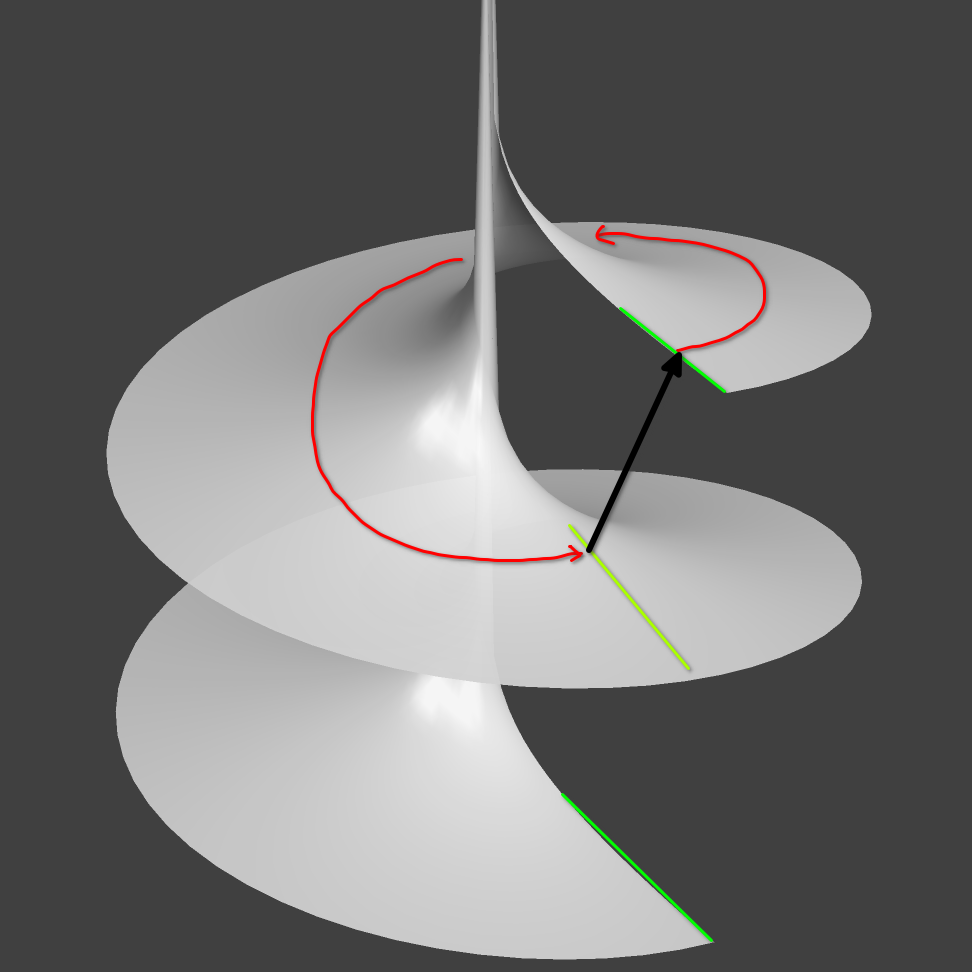
\includegraphics[width=0.9\textwidth]{RiemannSurfacePainted.png}
                \caption{黎曼面上的路径}
                \label{fig:riemann_surface_painted}
            \end{minipage}
        \end{figure}

        黎曼面实际上就是对多值函数定义域的扩充,再看看我们的老朋友$f(z) = \sqrt{z - z_0}$,因为它将点$z$映射到了两个点
        $\pm \sqrt{|z - z_0|}e^{i\frac{\theta}{2}}$上,所以它并不是严格的函数,为了将其变为单值函数,我们只要取两个复平面,
        将定义域铺在这两个复平面上,这样就能避免一对二的情况.

        多值函数$f(z) = \sqrt{z - z_0}$的黎曼面就类似图\ref{fig:riemann_surface}所示,但实际上在三维空间中我们没办法画出黎曼面的准确形状,
        因为你需要用某种神秘力量把图\ref{fig:riemann_surface_painted}中的上下两条绿线粘在一起.

        \begin{definition}[Riemann Sheet]
            黎曼面上的每个平面被叫做黎曼叶(Riemann Sheet),多值函数在单个黎曼叶上是解析的单值函数.图\ref{fig:riemann_surface}中的黎曼面叫做双叶黎曼面,
            因为它是由两个复平面拼接而成的,同理,由几个复平面拼接成的黎曼面就叫做几叶黎曼面.
        \end{definition}

        观察图\ref{fig:riemann_surface_painted},我们让$z$沿红线由三楼向下走,对于多值函数$f(z) = \sqrt{z - z_0}$,
        每当$z$经过一次绿线时,函数值都会加一个负号,而当$z$走到一楼的绿线时,它就会被超时空传送回三楼的绿线处,
        也就是函数值回归到初始值,这就是黎曼面的一个特性,也就是说函数值在黎曼面上是周期的.

        同样,我们也可以很容易地画出$f(z) = \ln{z}$的黎曼面,它和\ref{fig:riemann_surface}差不多,但它是无限叶的,
        每经过一次绿线,函数值都会加(减)一个$2\pi i$.

        \begin{definition}
            若$z$绕分支点$z_0$在黎曼面上旋转$n$圈后,函数值回归初始值,那么我们就将$z_0$称为$n - 1$阶分支点.
        \end{definition}

        \begin{example}
            \label{ex:riemann_surface}
            指出多值函数$f(z) = \sqrt{(z + 1)(z - 2)}$的分支点及其类型.
        \end{example}
        \begin{solution}
            根式的可能分支点在$\infty$和根式内多项式的零点处.
            \begin{enumerate}[(a)]
                \item $z = -1$;在此点领域内任取一点 $z_1 = -1 + \rho_1 e^{i \phi_1}(\rho_1 \ll 1)$,有:
                    \begin{align*}
                        \sqrt{(z + 1)(z - 2)} = \sqrt{\rho_1 e^{i \phi_1}(-3 + \rho_1 e^{i \phi_1})} 
                        \approx \sqrt{-3 \rho_1}e^{i\frac{\phi_1}{2}}
                    \end{align*}
                    当$\phi_1$变为$\phi_1 + 2\pi$,即绕$z = -1$一周时,有:
                    \begin{align*}
                        \sqrt{(z + 1)(z - 2)} \approx \sqrt{-3 \rho_1}e^{i\frac{\phi_1 + 2\pi}{2}}
                        = -\sqrt{-3 \rho_1}e^{i\frac{\phi_1}{2}}
                        \neq \sqrt{-3 \rho_1}e^{i\frac{\phi_1}{2}}
                    \end{align*}
                    而当$\phi_1 + 2\pi$变为$\phi_1 + 4\pi$,即再绕$z = -1$一周时,有:
                    \begin{align*}
                        \sqrt{(z + 1)(z - 2)} \approx \sqrt{-3 \rho_1}e^{i\frac{\phi_1 + 4\pi}{2}}
                        = \sqrt{-3 \rho_1}e^{i\frac{\phi_1}{2}}
                    \end{align*}
                    所以$z = -1$为一阶分支点.
                \item $z = 2$;过程同上,也为一阶分支点
                \item $z = \infty$;在其邻域内任取一点$z_2 = \rho_2 e^{i \phi_2}(\rho_2 \gg 1)$,有:
                    \begin{align*}
                        \sqrt{(z + 1)(z - 2)} \approx \rho_2 e^{i\phi_2}
                    \end{align*}
                    当$\phi_2$变为$\phi_2 + 2\pi$,即绕$z = \infty$一周时,仍有:
                    \begin{align*}
                        \sqrt{(z + 1)(z - 2)} \approx \rho_2 e^{i\phi_2 + 2\pi}
                        = \rho_2 e^{i\phi_2}
                    \end{align*}
                    函数值没有发生改变,所以$z = \infty$不是分支点.
            \end{enumerate}
        \end{solution}

        对于例\ref{ex:riemann_surface}中的函数,我们得到了它的两个分支点$z = -1$和$z = 2$,
        如果我们连接这两个分支点,我们会发现,每当$z$经过这条连线时,$f(z)$就会产生多值性,
        于是我们把这样的线称作割线,只要限制多值函数的自变量始终不越过割线,我们就能保证函数值的唯一性.
        

    \subsection{初等多值函数}
        本小节只作扩展,咱们在多值函数这方面并不会考这么多,只需要掌握根式下多项式形式的多值函数
        (即$\sqrt{(z - a_1)(z - a_2)\cdots(z - a_n)}$)分支点和割线的求法即可.

        \begin{enumerate}
            \item 一般幂函数$w = z^a = e^{a \ln{z}}$
                \begin{enumerate}[(1)]
                    \item 当$a$为整数$n$时,$w$为$z$的单值函数.
                    \item 当$a$为\ 待续... %TODO
                \end{enumerate}
        \end{enumerate}

\section{复变函数的积分}

    \subsection{复积分}
        \begin{definition}[复积分]\label{the:complex_integral}
            复积分可以简单定义为:
            \begin{align*}
                \int_{\alpha_1}^{\alpha_2}f(z)dz 
                = \lim_{\substack{N \to \infty \\
                \varDelta z_j \to 0}}
                \sum_{j = 1}^{N}f(z_j)\varDelta z_j
            \end{align*}
            其中,$\varDelta z_j$是在$z_j$处的小分割,$z_j$位于连接$\alpha_1, \, \alpha_2$的曲线上.
        \end{definition}

        我们可以将$f(z)$写作$f(z) = u + iv$,并且有$dz = dx + idy$,于是复积分也可以写作第二类曲线积分的形式方便计算.
        \begin{align}
            \int_{\alpha_1}^{\alpha_2}f(z)dz = \int_{\alpha_1}^{\alpha_2}(udx - vdy) + i \int_{\alpha_1}^{\alpha_2}(vdx + udy)
        \end{align}

        \begin{remark}
            数分中实变函数的积分中值定理并不能直接推广到复变积分上.
            \begin{align*}
                \int_{0}^{2\pi}e^{i\theta}d\theta = \int_{0}^{2\pi}\cos{\theta}d\theta + i \int_{0}^{2\pi}\sin{\theta}d\theta = 0
            \end{align*}
            而$e^{i\theta} \neq 0, \quad (0 < \theta < 2\pi)$
        \end{remark}

        计算复变函数的积分一般使用参数法,这样就能把多变量的积分转化成单变量的积分,我们更喜欢不那么复杂的计算.

        \begin{example}
            \label{ex:important_integral}
            这里给出一个常用复积分
            \begin{align*}
                \int_{C}\frac{dz}{(z - a)^n} = 
                \left\{
                    \begin{aligned}
                        2\pi i ,& \quad n = 1 \\
                        0 ,& \quad n \neq 1
                    \end{aligned}
                \right.
            \end{align*}
            $C$为以$a$为心,$\rho$为半径的圆周.积分值与$\rho,\ a$均无关.
        \end{example}
        \begin{proof}
            \label{proof:important_integral}
            将$C$写为参数形式$z - a = \rho e^{i\theta},\ 0 \leq \theta \leq 2\pi$.
            \begin{align*}
                \int_{C}\frac{dz}{(z - a)^n} = \int_{0}^{2\pi}\frac{i \rho e^{i\theta}d\theta}{\rho^n e^{in\theta}} = \int_{0}^{2\pi}\frac{id\theta}{\rho^{n - 1}e^{i(n-1)\theta}}
            \end{align*}
            当$n = 1$时我们很容易得到积分值为$2\pi i$,当$n \neq 1$时,我们有:
            \begin{align*}
                \int_{0}^{2\pi}\frac{id\theta}{\rho^{n - 1}e^{i(n-1)\theta}}
                &= \frac{i}{\rho^{n - 1}}\int_{0}^{2\pi}e^{-i(n-1)\theta}d\theta\\
                &= \frac{i}{\rho^{n - 1}}\left[ \int_{0}^{2\pi}\cos{(n - 1)\theta}d\theta - i \int_{0}^{2\pi}\sin{(n - 1)\theta}d\theta \right]\\
                &= 0
            \end{align*}
        \end{proof}

    \subsection{柯西定理}
        \begin{theorem}[Cauchy 定理]\label{the:cauchy_theorem}
            若$f:\mathbbm{C}\to\mathbbm{C}$在闭合曲线$C$及$C$内的所有点上解析,
            则有:
            \begin{align*}
                \oint_{C}f(z)dz = 0
            \end{align*}
        \end{theorem}

        由Cauchy定理我们可以得到如下引理:
        \begin{lemma}
            若$f(z)$在区域$G\subset\mathbbm{C}$上解析,则复积分$\int_{C}f(z)dz$的值
            与路径$C,\ (C \subset G)$无关.
        \end{lemma}

        下面两个引理对后续结论证明比较有用,可以记一下.
        \begin{lemma}
            \label{lem:small_arc_lemma}
            小圆弧引理:若函数$f(z)$在$z = a$点的空心领域内连续,且在$\theta_1 \leq \arg{(z - a)} \leq \theta_2$区域内时,
            有$\lim_{|z - a| \to 0}(z - a)f(z) \to k$,则
            \begin{align*}
                \lim_{\delta \to 0}\int_{C_\delta}f(z)dz = ik(\theta_2 - \theta_1)
            \end{align*}
            式中$C_\delta$是以$z = a$为圆心、$\delta$为半径、角度为$\theta_2 - \theta_1$的圆弧,
            $|z - a| = \delta,\,\theta_1 \leq \arg{(z - a)} \leq \theta_2$,如图\ref{fig:small_arc}所示.
        \end{lemma}

        \begin{figure}[htbp]
            \centering
            \begin{minipage}[t]{0.48\textwidth}
                \centering
                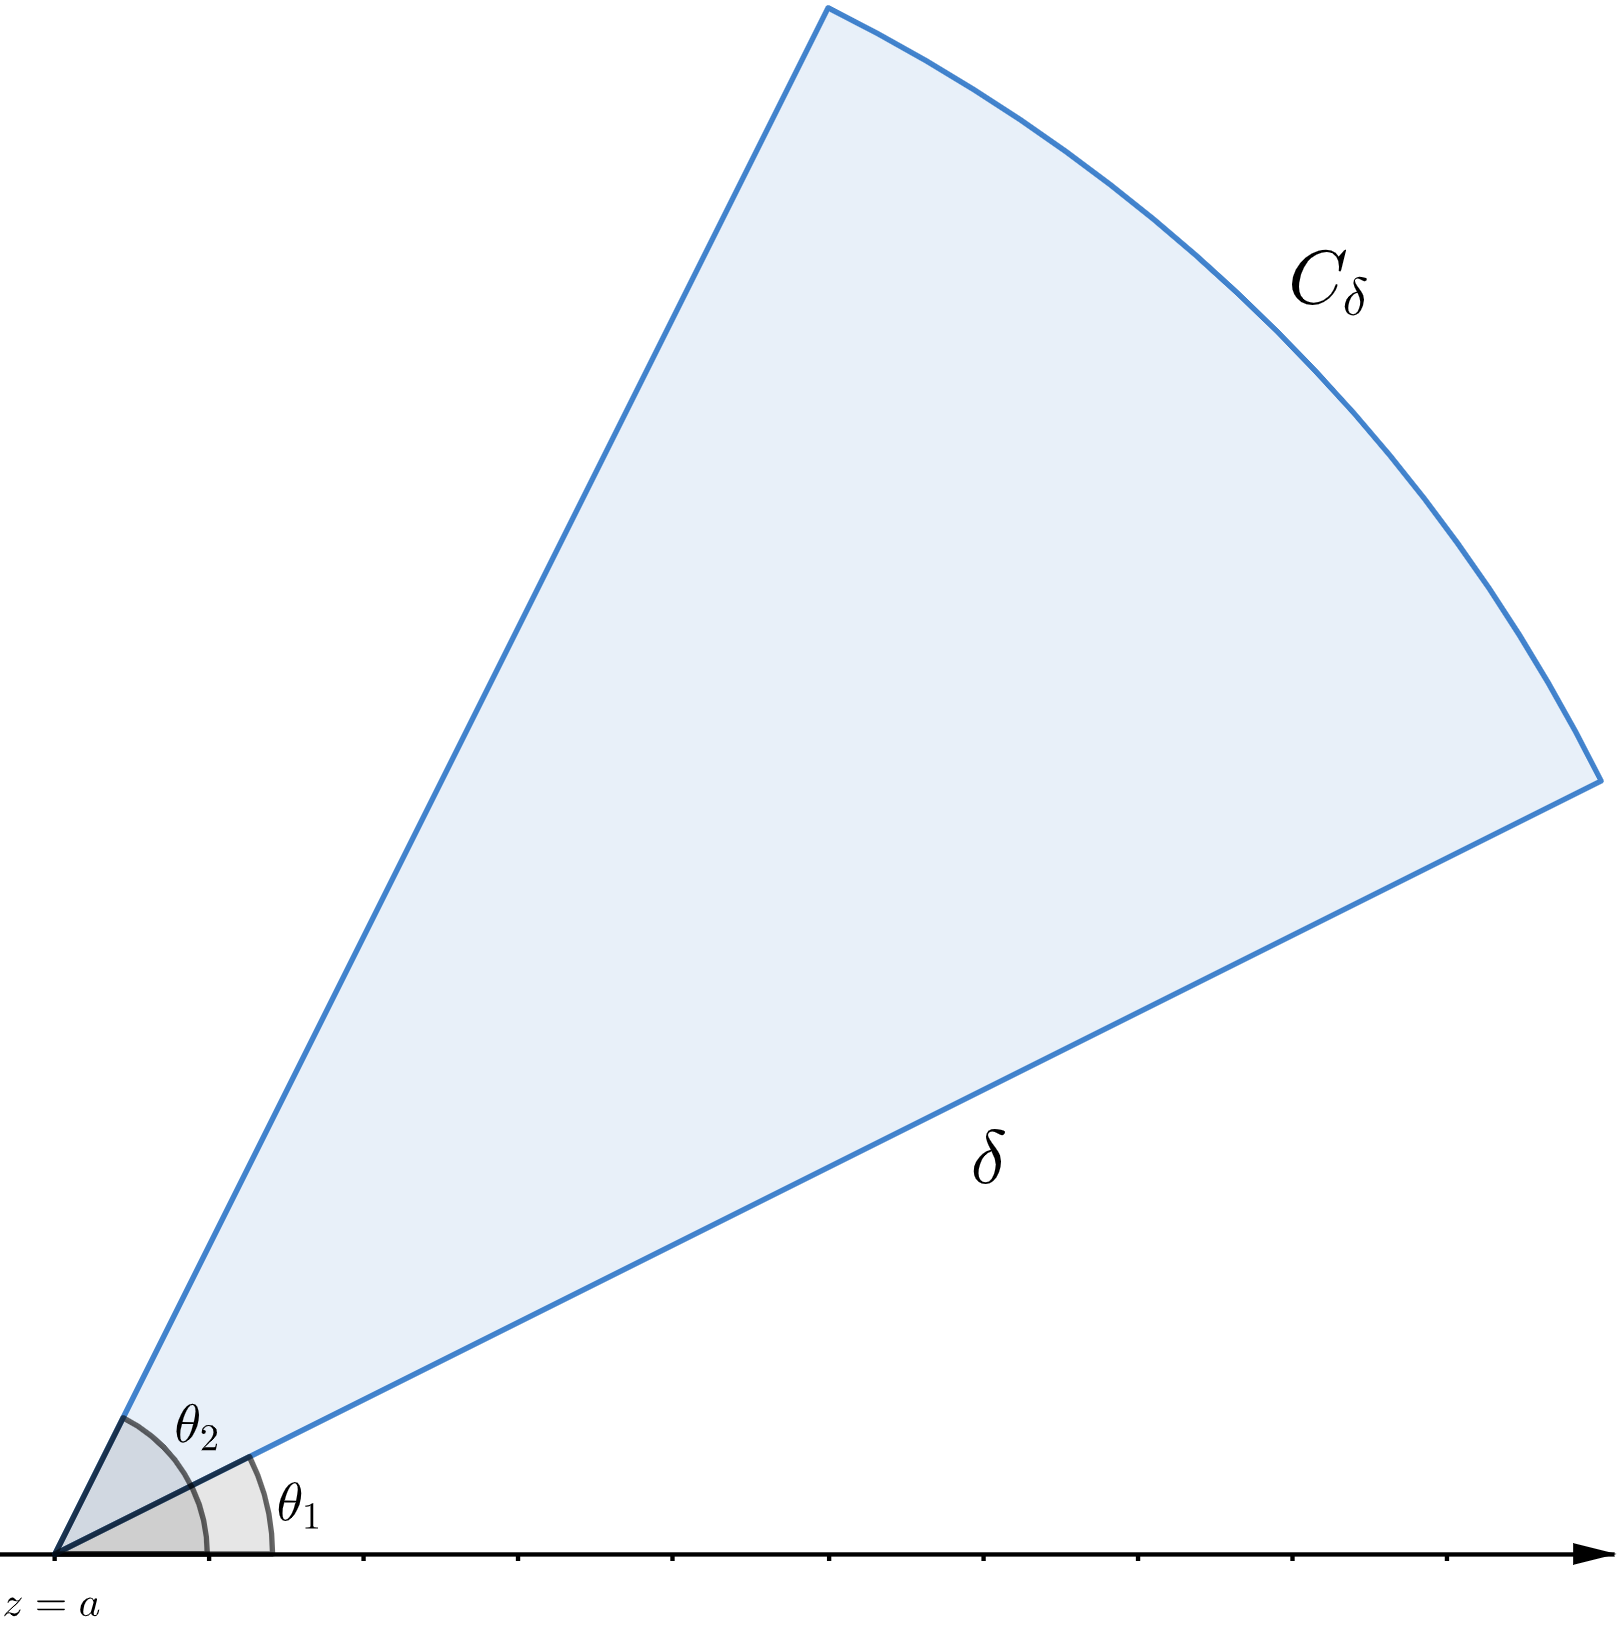
\includegraphics[width=0.9\textwidth]{SmallArc.png}
                \caption{小圆弧}
                \label{fig:small_arc}
            \end{minipage}
            \begin{minipage}[t]{0.48\textwidth}
                \centering
                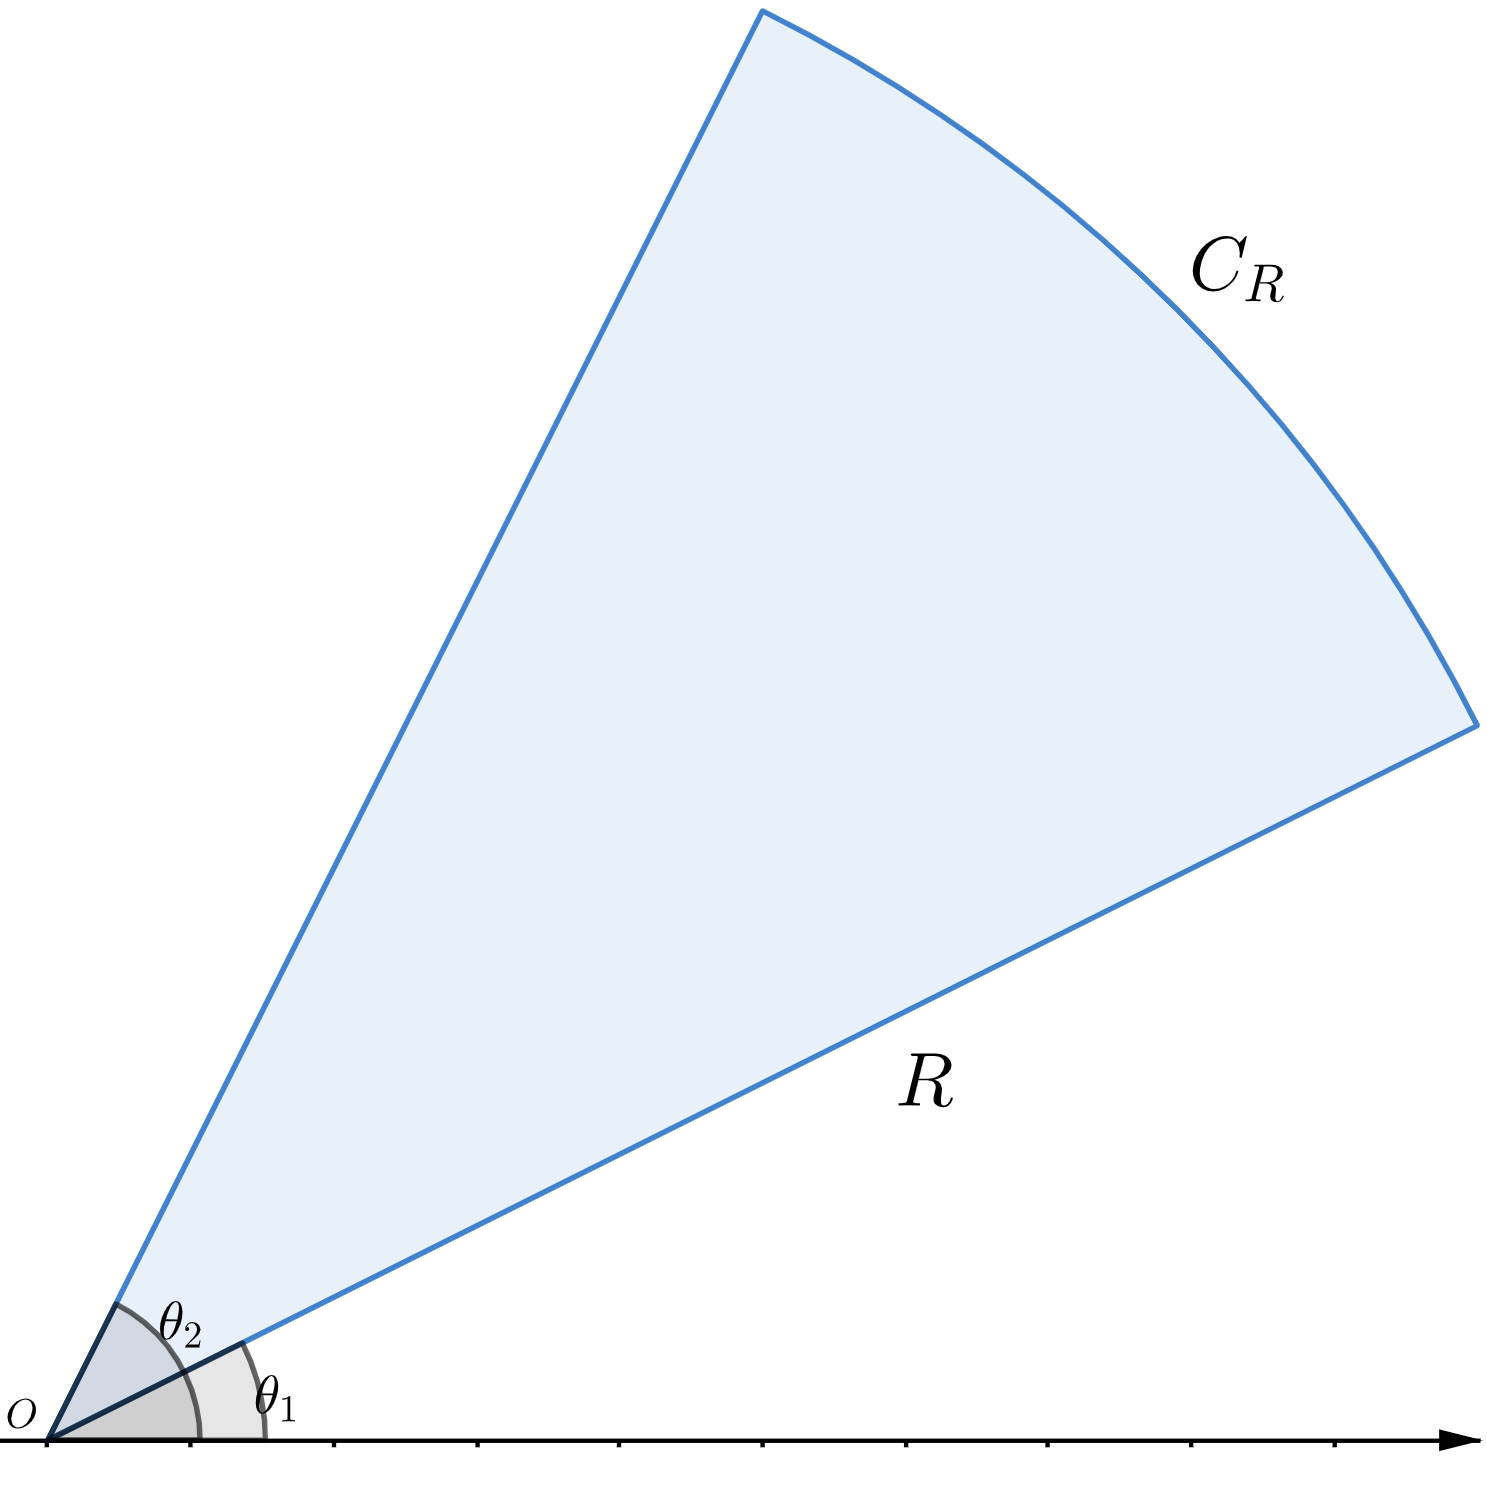
\includegraphics[width=0.9\textwidth]{LargeArc.png}
                \caption{大圆弧}
                \label{fig:large_arc}
            \end{minipage}
        \end{figure}

        \begin{lemma}
            \label{lem:large_arc_lemma}
            大圆弧引理:与小圆弧引理相似,若函数$f(z)$在$\infty$点的领域内连续,且在$\theta_1 \leq \arg{z} \leq \theta_2$区域内时,
            有$\lim_{|z| \to \infty}zf(z) \to K$,则
            \begin{align*}
                \lim_{R \to \infty}\int_{C_R}f(z)dz = iK(\theta_2 - \theta_1)
            \end{align*}
            式中$C_R$是以原点为圆心、$R$为半径、角度为$\theta_2 - \theta_1$的圆弧,
            $|z| = R,\,\theta_1 \leq \arg{z} \leq \theta_2$,如图\ref{fig:large_arc}所示.
        \end{lemma}

    \subsection{柯西积分公式}
        \begin{theorem}[Cauchy积分公式]\label{the:cauchy_integral_formula}
            (Cauchy Integral Formula,简称CIF)设函数$f:\mathbbm{C} \to \mathbbm{C}$
            在闭合曲线$C$上解析,则对$C$内任一个点$z = z_0$,都有
            \begin{align*}
                \label{eq:cauchy_integral_formula}
                f(z_0) = \frac{1}{2 \pi i}\oint_{C}\frac{f(z)}{z - z_0}dz
            \end{align*}
        \end{theorem}

        \begin{example}
            使用CIF求出下列三式的值
            \begin{align*}
                &I_1 = \oint_{C_1}\frac{z^2dz}{(z^2+3)^2(z-i)},
                \quad I_2=\oint_{C_2}\frac{(z^2-1)dz}{(z-\frac{1}{2})(z^2-4)^3},\\
                &I_3=\oint_{C_3}\frac{e^{\frac{z}{2}}dz}{(z-i\pi)(z^2-20)^4},
            \end{align*}
            $C_1,\ C_2,\ C_3$分别为以原点为圆心,以$r_1=\dfrac{3}{2},\ r_2=1,\ r_3=4$为半径的圆.
        \end{example}
        \begin{solution}
            对$I_1$,我们令$f(z) = \dfrac{z^2}{(z^2+3)^2}$,易见$f$在$C_1$及其内点上解析,
            在$C$内选取$z_0 = i$,由$CIF$我们有:
            \begin{align*}
                I_1=\oint_{C_1}\frac{f(z)dz}{z-i}=2\pi i f(i)=2\pi i\frac{i^2}{(i^2+3)^2}=-i\frac{\pi}{2}.
            \end{align*}

            同理,对于$I_2$我们取$f(z) = \dfrac{z^2 - 1}{(z^2 - 4)^3},\ z_0 = i$.
            \begin{align*}
                I_2 = \oint_{C_2}\frac{f(z)dz}{z - \frac{1}{2}} = 2\pi i f(\frac{1}{2}) = \frac{32\pi}{1125}i.
            \end{align*}

            对于$I_3$我们取$f(z) = \frac{e^{z/2}}{(z^2 - 20)^4},\ z_0 = i\pi$.
            \begin{align*}
                I_3 = \oint_{C_3}\frac{f(z)dz}{z-i\pi}=2\pi i f(i\pi) = -\frac{2\pi}{(\pi^2+20)^4}.
            \end{align*}
        \end{solution}

    \subsection{解析函数的高阶导数}
        我们先将$CIF$写成如下形式:
        \begin{align*}
            f(z) = \frac{1}{2\pi i}\int_C \frac{f(\xi)d\xi}{\xi - z}.
        \end{align*}

        \begin{theorem}[解析函数的高阶导数]\label{the:analytic_function_derivative}
            对上式求$n$阶导我们可以得到解析函数的$n$阶导公式:
            \begin{align*}
                f^{(n)}(z) = \frac{d^n f}{dz^n} = \frac{n!}{2\pi i}\oint_C \frac{f(\xi)d\xi}{(\xi - z)^{n + 1}}
            \end{align*}
        \end{theorem}

        我们将如下形式的积分称为柯西型积分:$$\oint_C \frac{g(\xi)d\xi}{p(\xi)}$$
        其中$p(z)$为关于$\xi$的多项式,即$p(\xi) = a_n(\xi - z_1)(\xi - z_2)\cdots(\xi - z_n)$.
        柯西型积分的求解有十分甚至九分简单,简要来说就是找处在$C$内的奇点,并确定函数$f(\xi)$和阶数,
        通过下例我们可以更加直观的理解柯西型积分的求解过程.
        \begin{example}
            求解柯西型积分
            \begin{align*}
                \oint_{|z + 1| = 1}\frac{dz}{(z + 1)^2(z - 2)}.
            \end{align*}
        \end{example}
        \begin{solution}
            $z = -1$为$|z + 1| < 1$内的一个奇点,$\dfrac{1}{z - 2}$在$|z + 1| < 1$内解析,
            由定理\ref{the:analytic_function_derivative},我们有
            \begin{align*}
                \oint_{|z + 1| = 1}\frac{\frac{1}{z - 2}}{(z + 1)^2}dz = 2\pi i\left( \frac{1}{z - 2} \right)'\Bigg|_{z=-1} = -\frac{2}{9}\pi i
            \end{align*}
        \end{solution}